The Earth-center, Earth-fixed(ECEF) frame:


In specific time origins of ECEF fix to earth centered inertial(ECI) frame and we assume in 100 second they don't change too much so we neglect this change.


$u^i(t) = u^i_o + a^i_xt,\quad v^i(t) = a^i_yt, \quad w^i(t) = 0$



$u_o^i = 100 ft/s,\quad a_x^i = 25 ft/s^2, \quad a_y^i = 50ft/s^2$

$$u^i(t) = 100 + 25t,\quad v^i(t) = 50t, \quad w^i(t) = 0$$
$$x^i(t) = 100t + 25/2t^2,\quad v^i(t) = 50/2t^2, \quad w^i(t) = 0$$

Figures have plot in MATLAB and code(Q1\_a) attached to home work file.
\begin{figure}[H]
	\caption{X location ECEF frame}
	\centering
	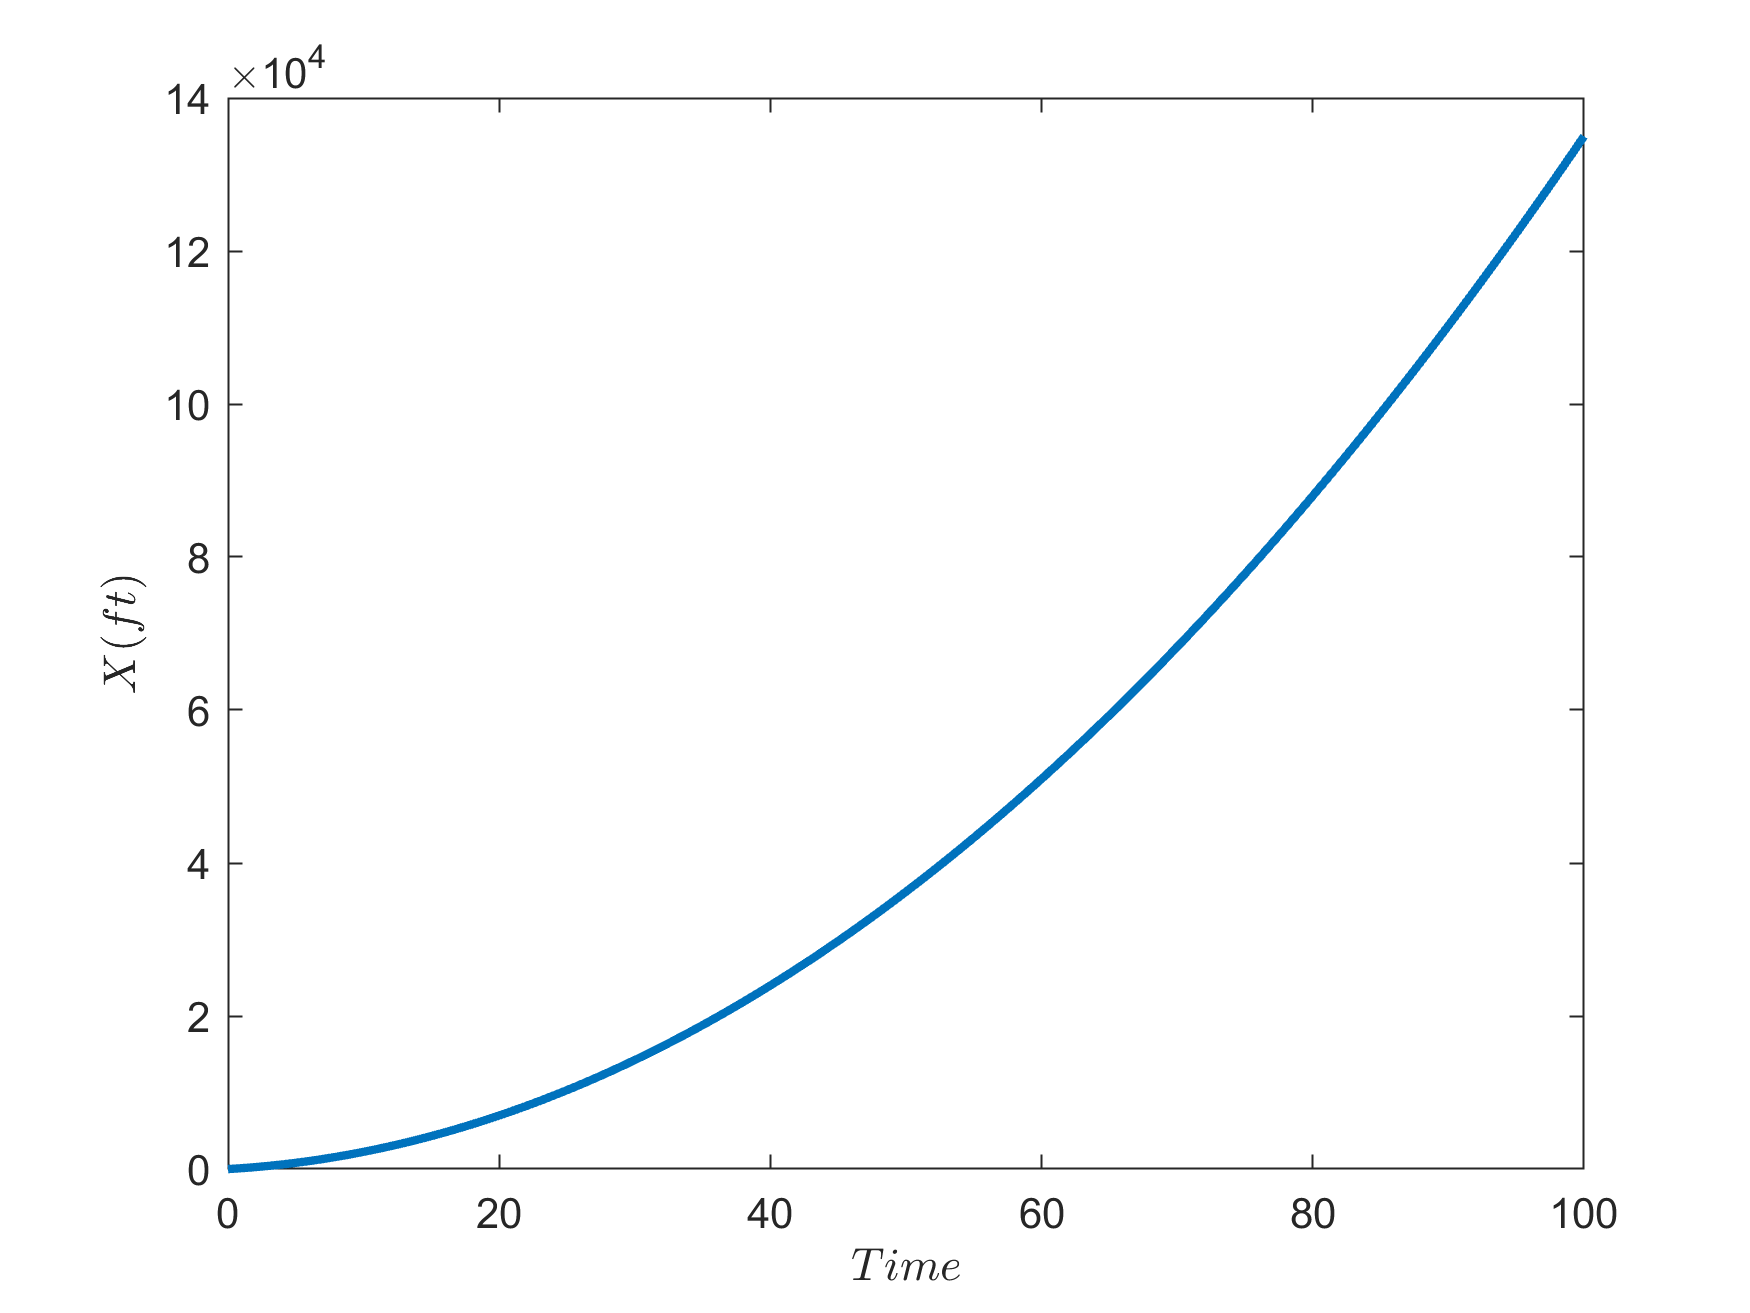
\includegraphics[width=12cm]{Q1/figures/X location.png}
\end{figure}
\begin{figure}[H]
	\caption{Y location ECEF frame}
	\centering
	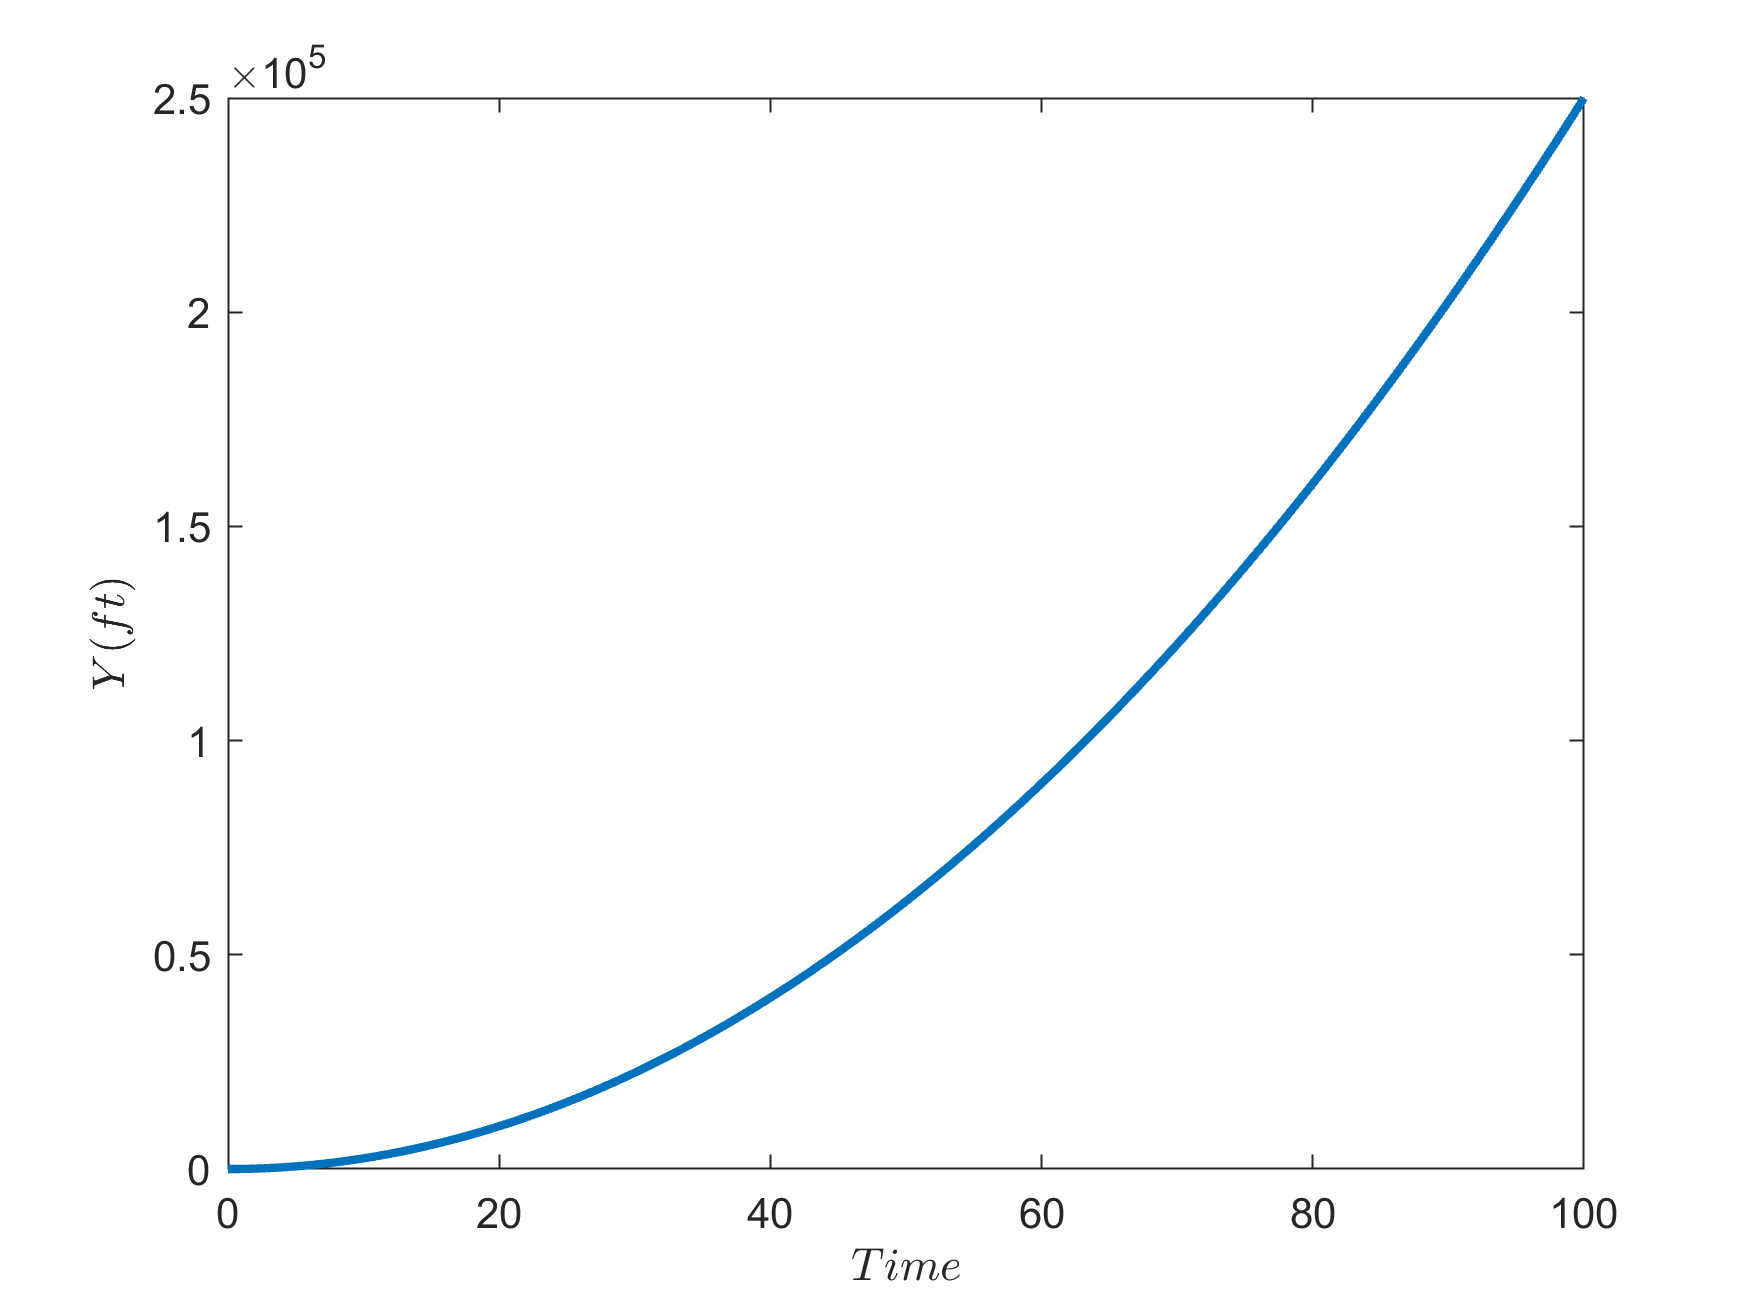
\includegraphics[width=12cm]{Q1/figures/Y location.png}
\end{figure}
\begin{figure}[H]
	\caption{Z location ECEF frame}
	\centering
	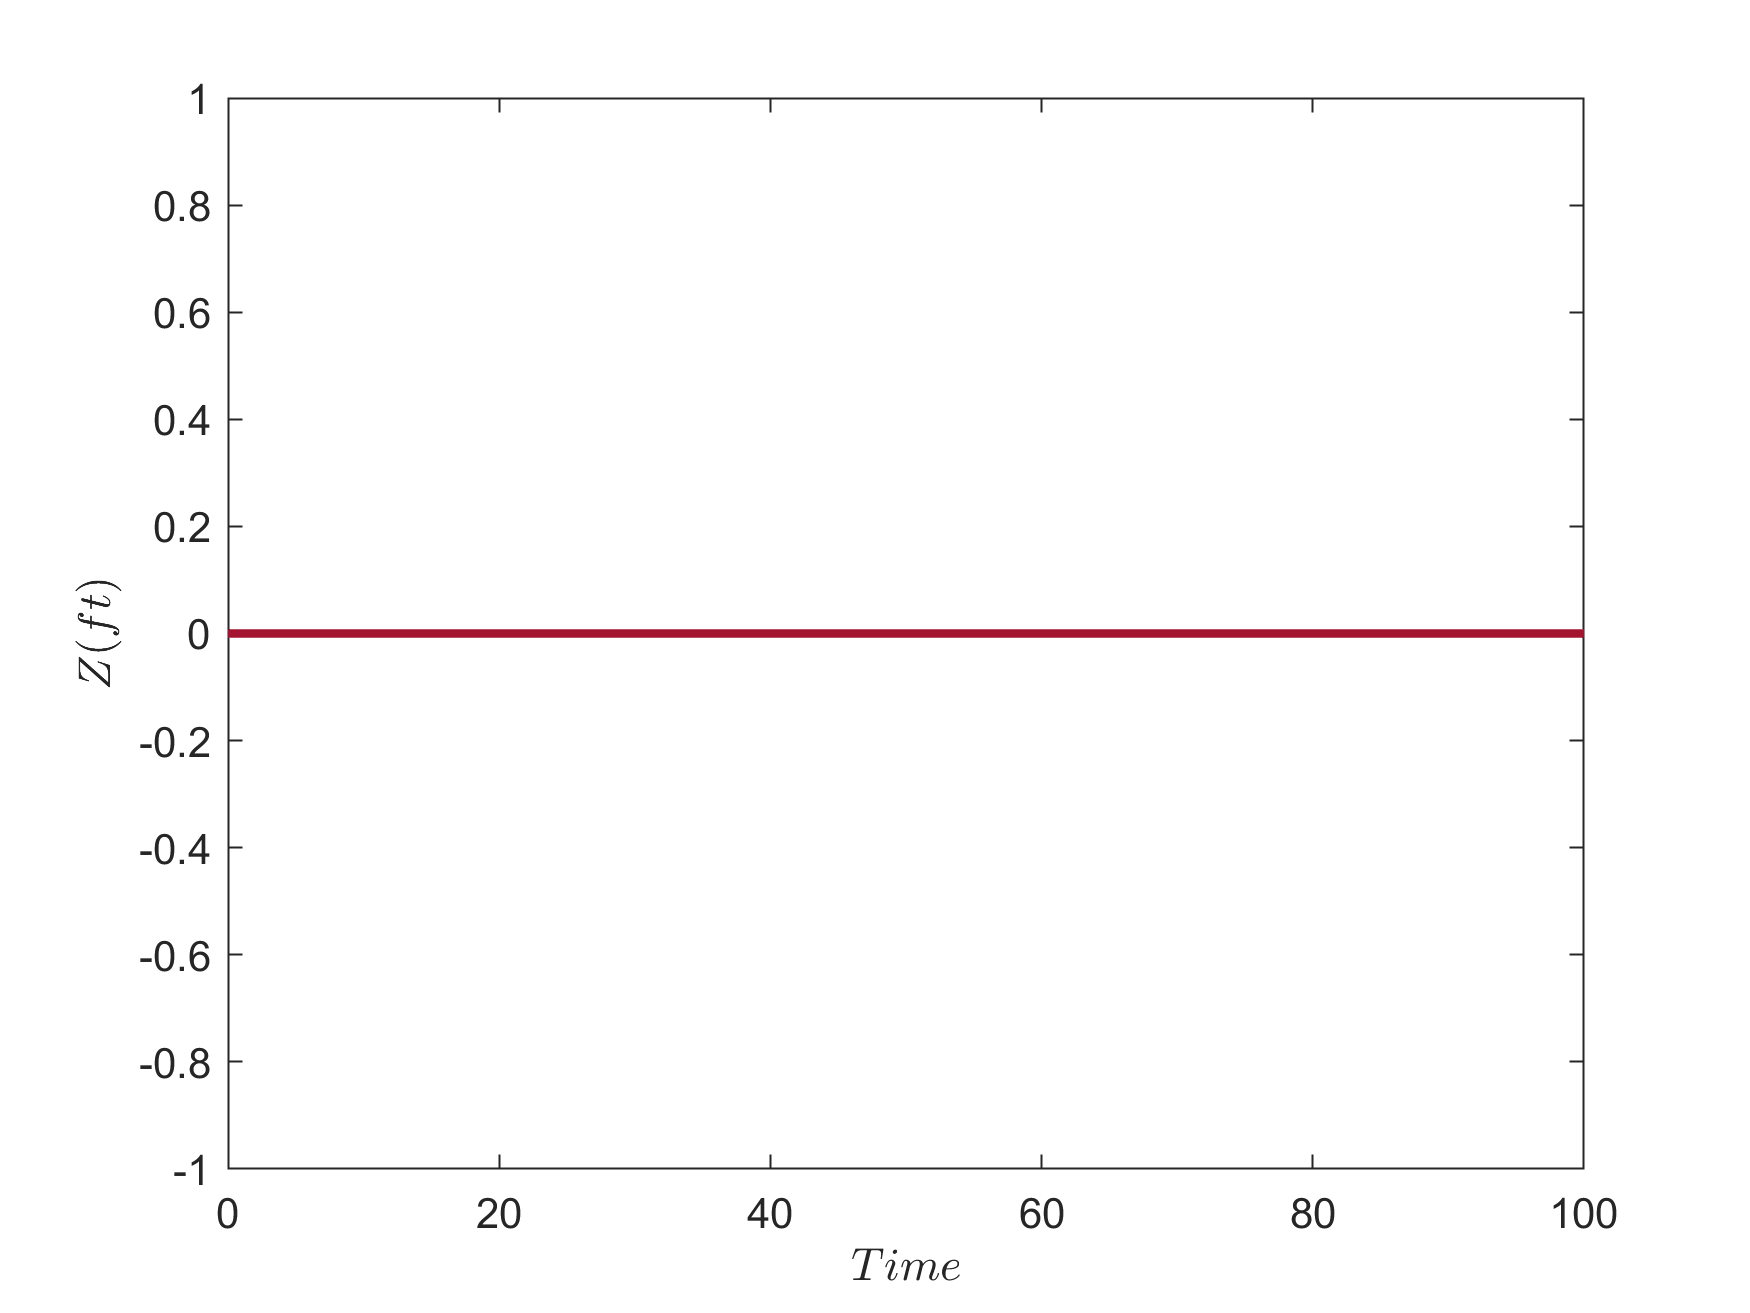
\includegraphics[width=12cm]{Q1/figures/Z location.png}
\end{figure}
\begin{figure}[H]
	\caption{X direction velocity ECEF frame}
	\centering
	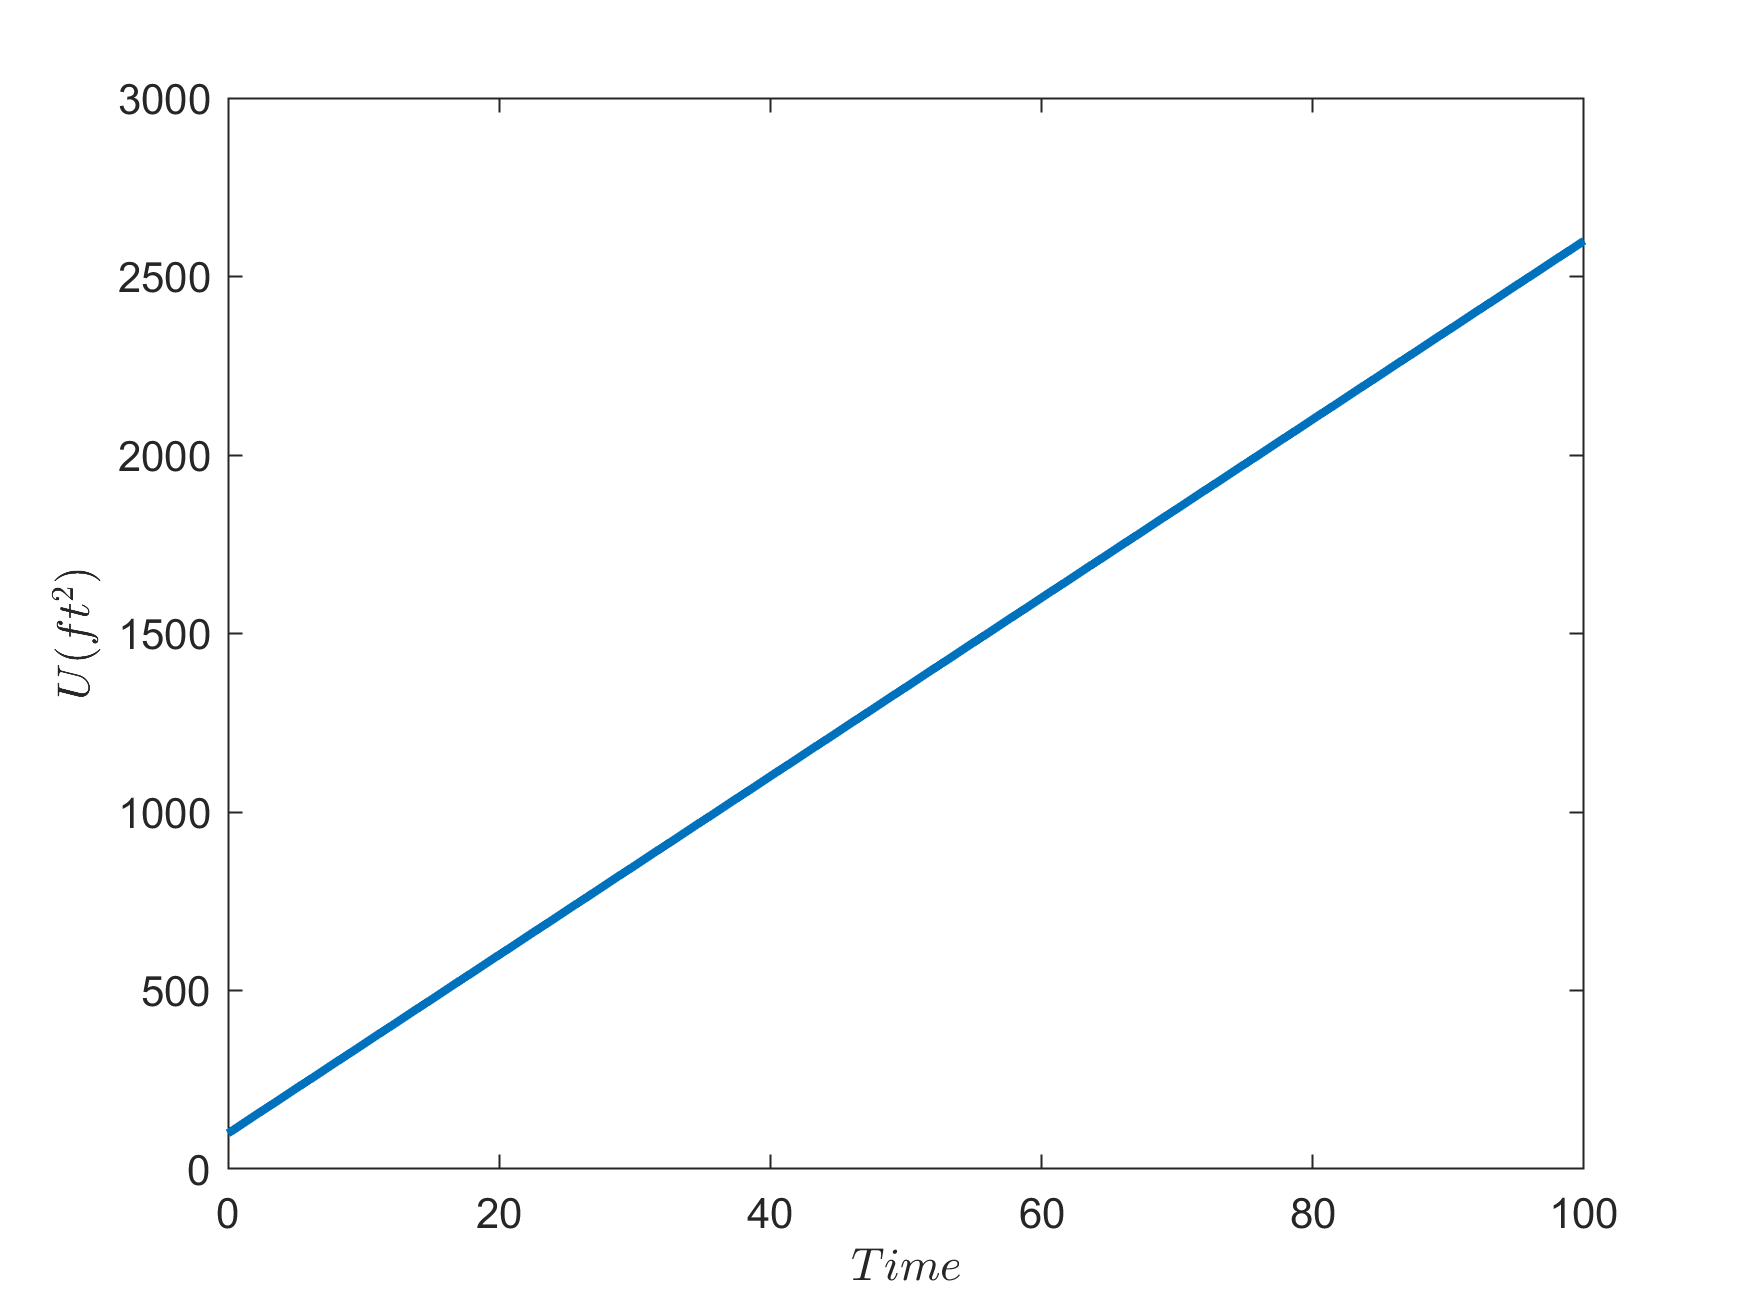
\includegraphics[width=12cm]{Q1/figures/X velocity.png}
\end{figure}
\begin{figure}[H]
	\caption{Y direction velocity ECEF frame}
	\centering
	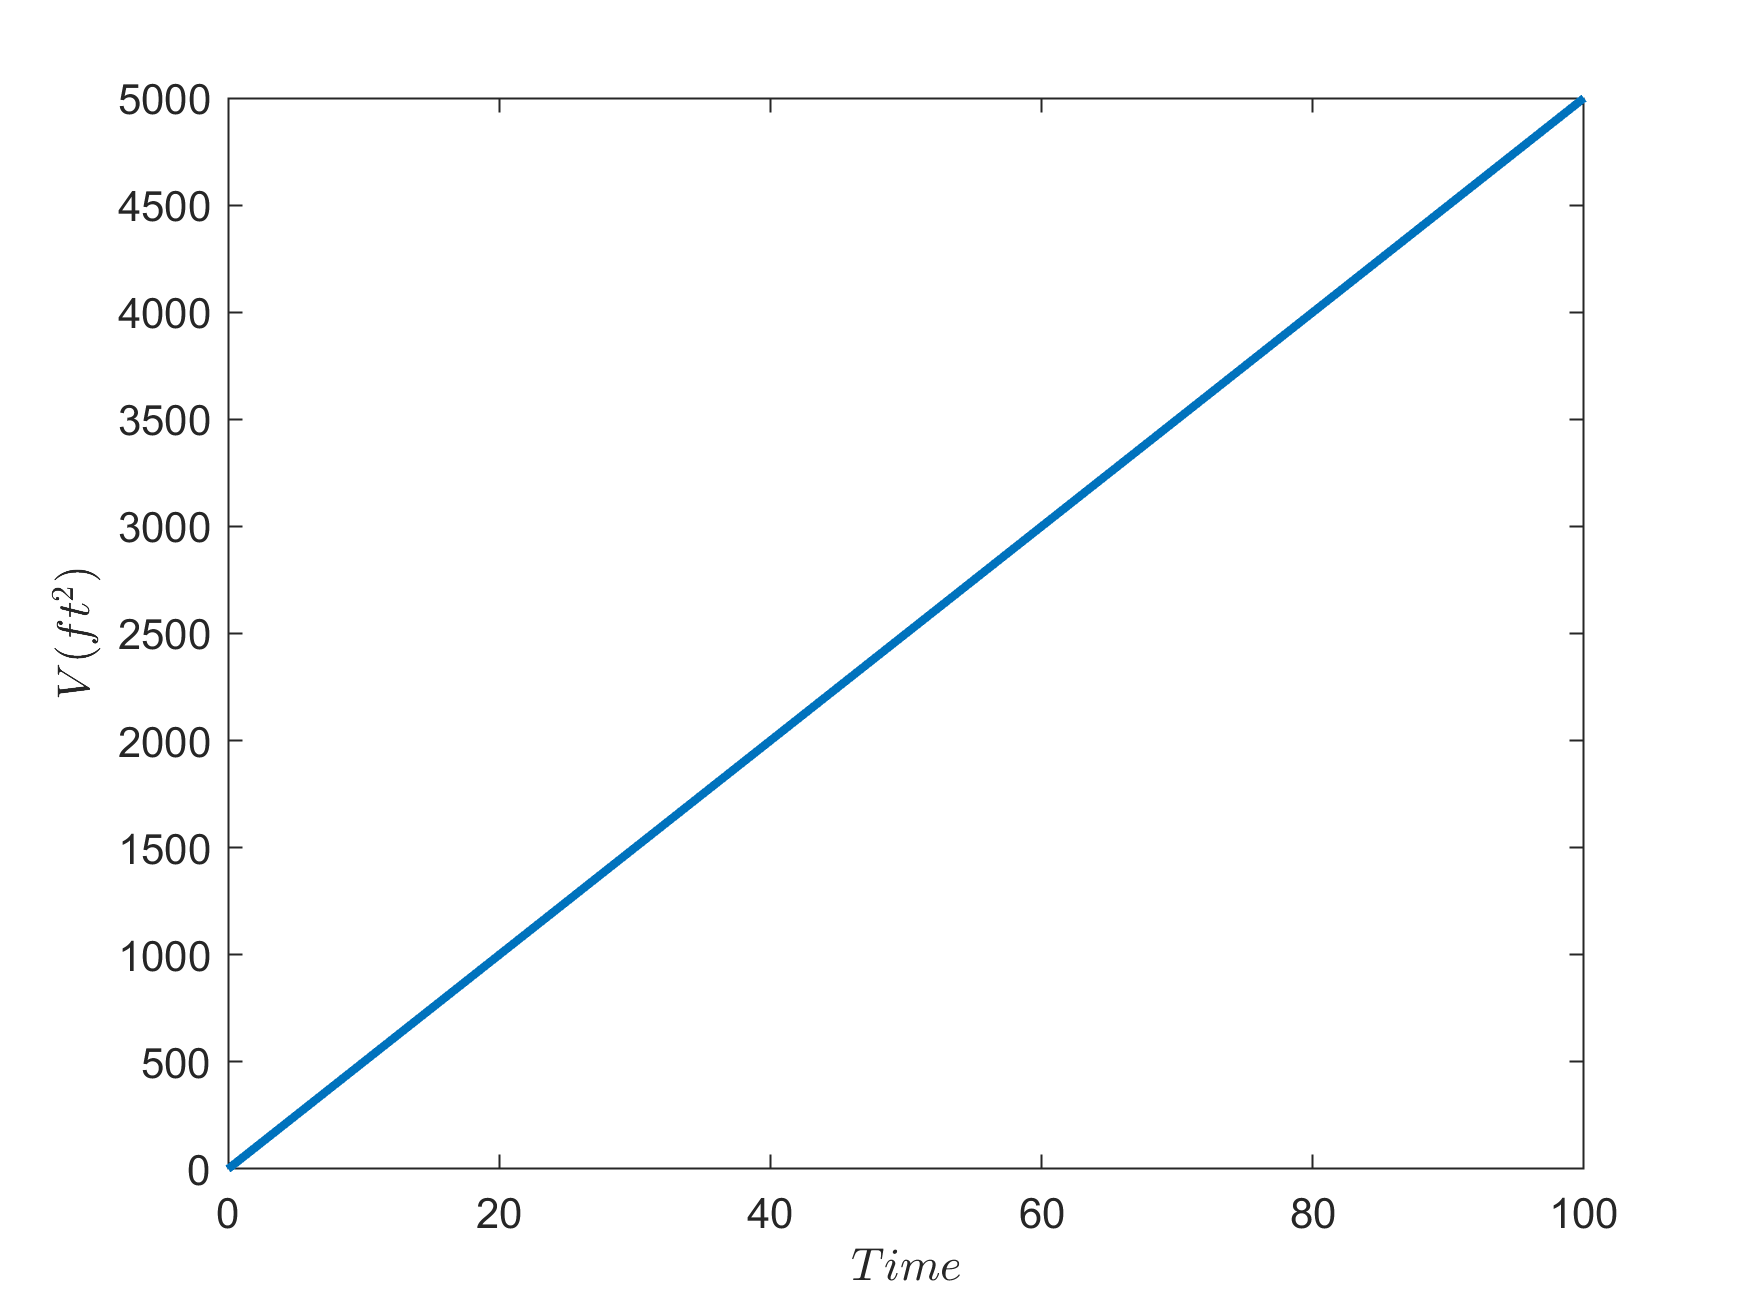
\includegraphics[width=12cm]{Q1/figures/Y velocity.png}
\end{figure}
\begin{figure}[H]
	\caption{Z direction velocity ECEF frame}
	\centering
	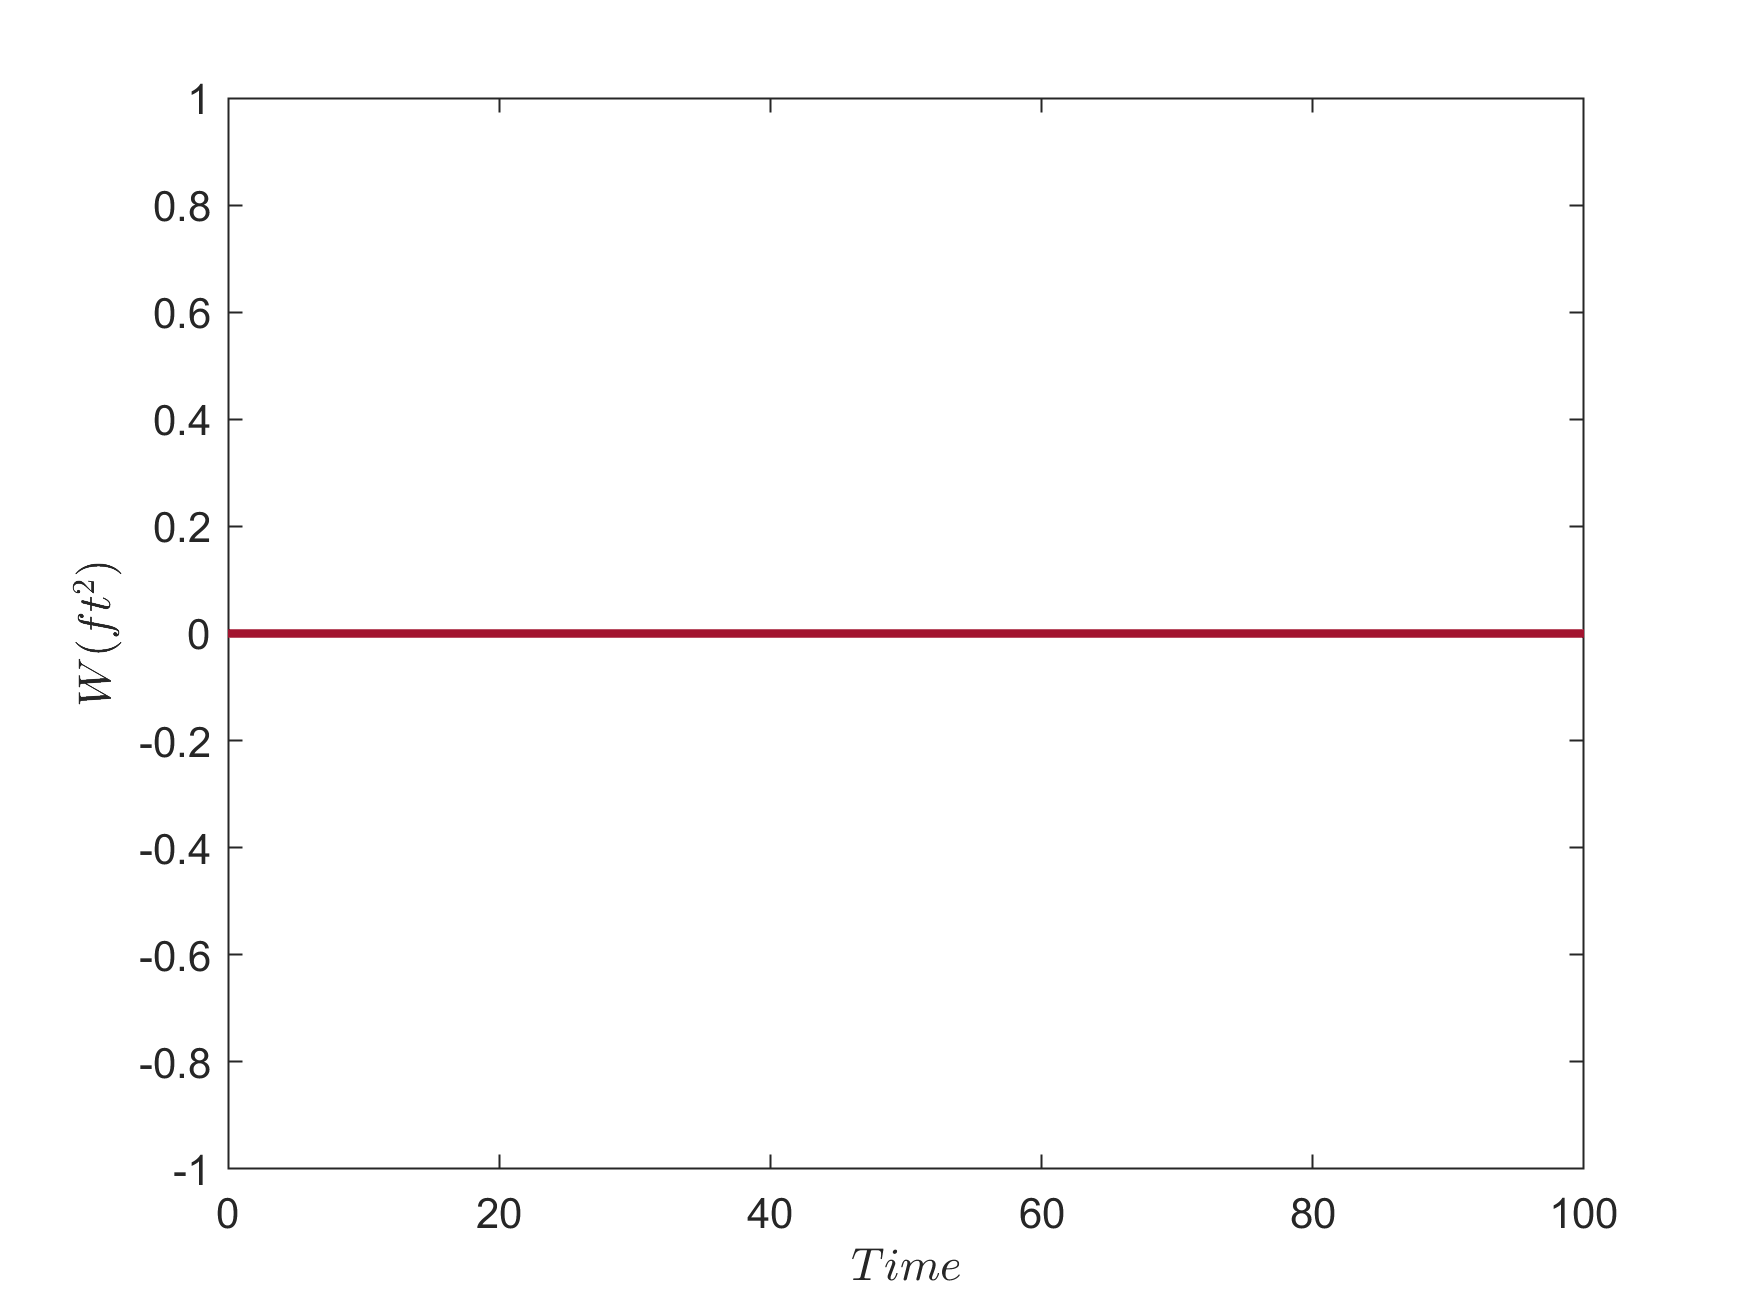
\includegraphics[width=12cm]{Q1/figures/Z velocity.png}
\end{figure}